\chapter{Risultati Sperimentali}
\label{cap:risultati}

Nel seguente capitolo discuteremo i risultati sperimentali ottenuti con il presente lavoro di tesi.

Nel Capitolo~\ref{cap:prototipo} abbiamo sviluppato un prototipo di videogioco completo basato su Unity DOTS, il quale ci è servito per approfondire le librerie da un punto di vista high-level. In particolare, le funzionalità realizzate lo rendono un progetto completo ed un gioco a tutti gli effetti. Oltre a questo prototipo, per valutare gli aspetti legati alle performance, ne abbiamo sviluppato uno ad hoc per il testing.

Prima di proseguire con l'analisi dei risultati sperimentali, introduciamo alcuni degli strumenti utilizzati per la valutazione.

Lo sviluppo del prototipo ed i relativi test sono stati eseguiti sulla seguente architettura:
\begin{itemize}
    \item Processore Intel(R) Core(TM) i7-7700HQ con 4 core (8 processori logici) e frequenza di clock pari a 2.80GHz.
    \item Memoria RAM da 16GB.
    \item Scheda video NVIDIA GeForce GTX 1060.
    \item Sistema Operativo Microsoft Windows 10 Home, a 64 bit.
\end{itemize}

Per poter analizzare le varie informazioni del sistema, possiamo sfruttare il Profiler Unity (vedi Figura~\ref{fig:prototipo-profiler}. Questo è uno strumento compreso nell'editor, che ci permette esaminare alcuni dei dati pratici: nella parte superiore possiamo vedere il carico sulla CPU dei vari componenti dell'applicazione; nella parte inferiore possiamo vedere dove eseguono effettivamente le parti del nostro codice. Partendo dall'alto verso il basso si costruisce una gerarchia di gruppi e sistemi di esecuzione, dove il più esterno è il ciclo del PlayerLoop, ovvero l'esecuzione dell'applicazione

\begin{figure}[!ht]
    \centering
    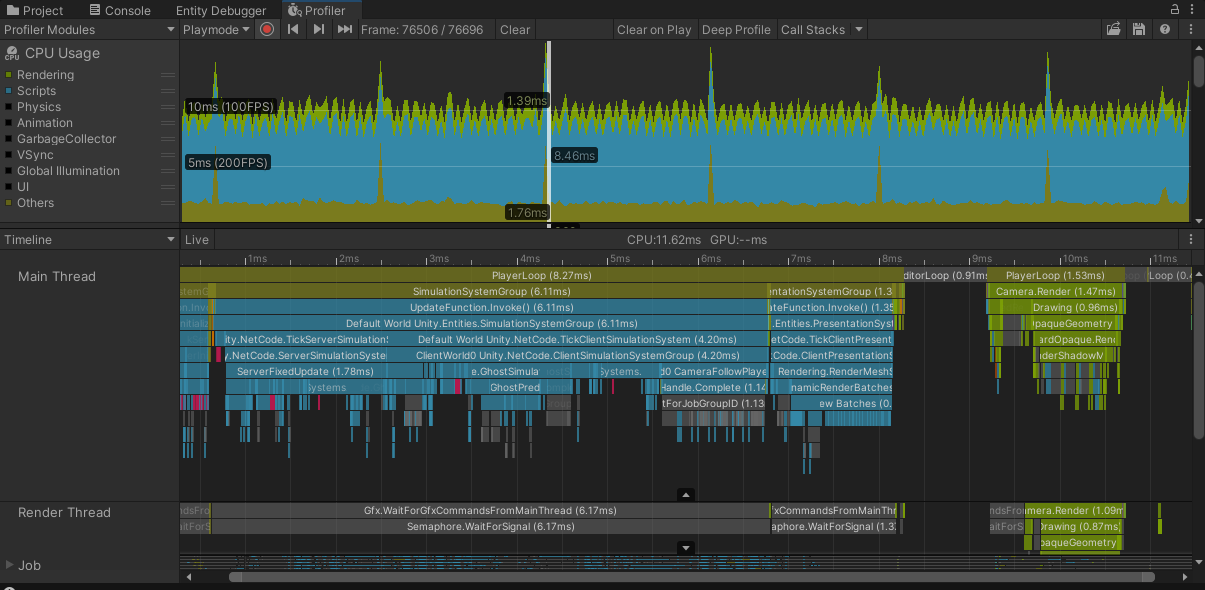
\includegraphics[width=0.95\columnwidth]{gfx/imgs/chapter5/ProfilerPrototipo.png}
    \caption{Profiler Unity: un frame durante l'esecuzione.}
    \label{fig:prototipo-profiler}
\end{figure}


\section{Valutazione performance DOTS}

Per la realizzazione del prototipo sono state costruite due scene, una per il test riguardante l'architettura classica e una per i test relativi ad ECS, Jobs e Burst. In entrambe le scene è presente il medesimo GameObject, il quale è associato ad un componente ``spawner''. Questo componente permette, in base a dei campi modificabili, di creare un numero arbitrario di cubi. Nella prima scena i cubi sono costituiti da GameObject, mentre nella seconda sono costituiti da entità. Gli oggetti creati sono in entrambi i casi dei cubi con una grafica a righe gialle e nere, in modo tale che sia possibile vederne il movimento. Una volta istanziati, i cubi vengono fatti ruotare all'interno della scena. Nel caso dell'architettura classica, la rotazione avviene tramite un MonoBehaviour associato al GameObject del cubo; mentre nel caso di ECS, la rotazione è realizzata da un sistema.

Durante la fase di testing, abbiamo eseguito il prototipo sfruttando diverse configurazioni, ovvero:

\begin{itemize}
    \item Architettura classica, tramite lo spawn di GameObject e rotazione di questi tramite MonoBehaviour.
    \item ECS ``vanilla'', tramite lo spawn di entità e la rotazione di queste aggiornando un sistema sul main thread.
    \item ECS e job, come il precedente ma scheduliamo la \verb|OnUpdate()| del sistema affinché venga eseguita su un singolo worker thread;
    \item ECS e job paralleli, come il precedente, ma scheduliamo diversi job che eseguiranno in parallelo sui worker thread;
    \item ECS e job paralleli, come il precedente ma compilando i job con Burst.
\end{itemize}

La tabella in Figura~\ref{fig:dati-stress-test} riporta i dati rilevati durante le prove:

\begin{figure}[!ht]
    \centering
    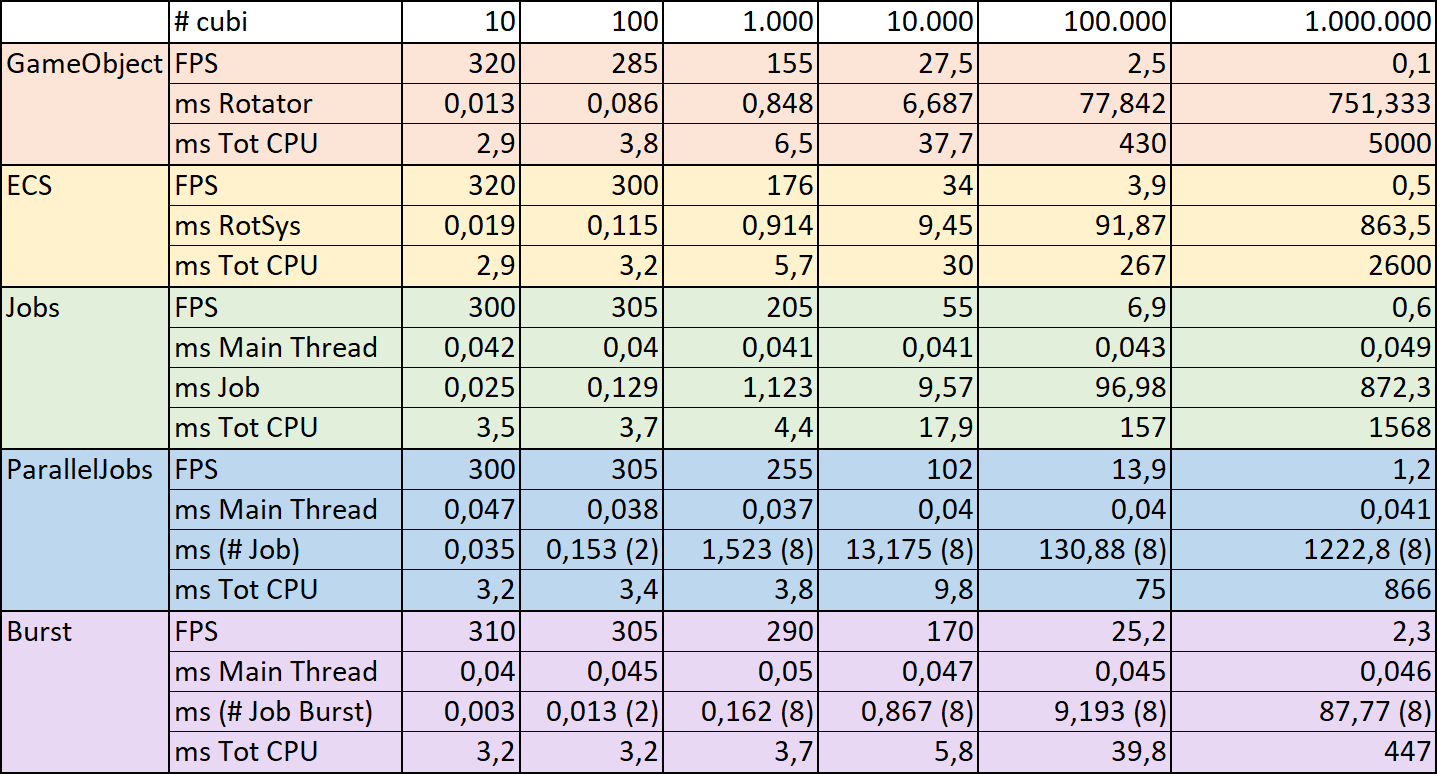
\includegraphics[width=0.95\columnwidth]{gfx/imgs/chapter5/RaccoltaDati.png}
    \caption{Raccolta dati}
    \label{fig:dati-stress-test}
\end{figure}

In particolare, per ogni test abbiamo riportato:
\begin{itemize}
    \item FPS dell'applicazione durante l'esecuzione.
    \item Tempo in millisecondi impiegato dal MonoBehaviour o dai sistemi per ruotare tutti gli oggetti. Nel caso di Jobs, ParallelJobs e Burst, questo valore viene suddiviso fra main thread e worker thread.
    \item Tempo totale in millisecondi impiegato dalla CPU per eseguire un frame completo.
\end{itemize}

Per ottenere i risultati in tabella, abbiamo eseguito il prototipo una volta per ciascuna configurazione. Ad ogni esecuzione abbiamo campionato 10 frame. Dopodiché, per ognuno di questi, abbiamo salvato i valori di FPS e millisecondi, e successivamente calcolato la loro media. Queste operazioni sono poi state ripetute incrementando il numero di cubi creati, come riportato in tabella.

Nelle prossime sezioni approfondiremo i risultati ottenuti per ognuna delle configurazioni testate.

\subsubsection{Architettura classica}
Nel caso dell'architettura classica, vengono prima creati dei GameObject. Successivamente, questi ultimi vengono messi in rotazione per mezzo del MonoBehaviour che posseggono. In particolare, questa rotazione avviene all'interno del metodo \verb|Update()|. Infatti, tramite il profiler possiamo notare come questa funzione venga eseguita per ognuno dei cubi presenti in scena. Sempre grazie al profiler, possiamo vedere come ogni rotazione avvenga in sequenza nel main thread. Se osserviamo il grafico in Figura~\ref{fig:profiler-100k(1)}, vediamo che le 100.000 istanze del MonoBehaviour \verb|Rotator| impiegano circa 76,5 ms per ruotare i GameObject; mentre facendo riferimento alla Figura~\ref{fig:dati-stress-test}, notiamo che l'applicazione viene eseguita con una media di 2,5 FPS.

\begin{figure}[!ht]
    \centering
    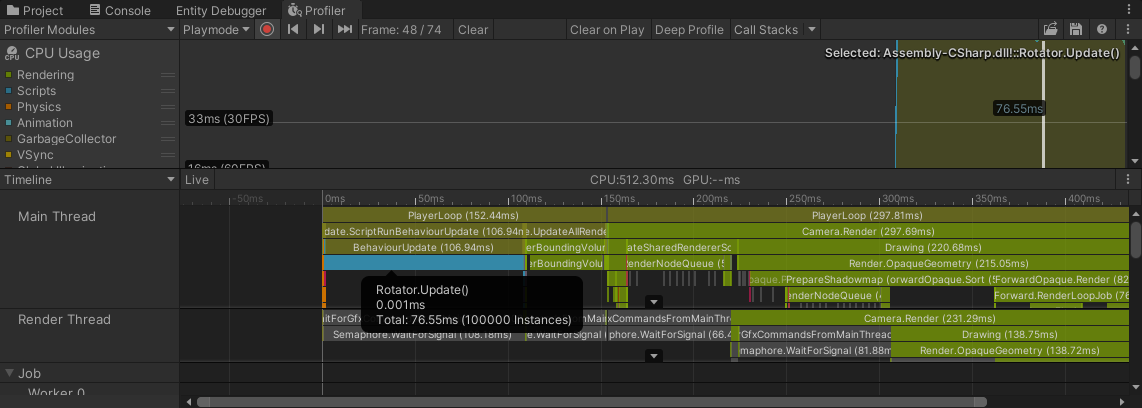
\includegraphics[width=0.95\columnwidth]{gfx/imgs/chapter5/ProfilerStressTest100k(1).png}
    \caption{Profiler: rotazione di 100.000 GameObject tramite un MonoBehaviour.}
    \label{fig:profiler-100k(1)}
\end{figure}

\subsubsection{ECS}
Per i test con ECS abbiamo realizzato un componente \verb|RotateComponent| ed un sistema \verb|RotatorSystem|. Questo componente viene assegnato alle entità dei cubi non appena vengono creati.

Nel test in questione, all'interno del metodo \verb|OnUpdate()| del sistema, eseguiamo la lambda expression che itera sulle entità tramite \verb|Run()|. Così facendo la funzione verrà eseguita sul main thread. Come si può notare in Figura~\ref{fig:profiler-100k(2)}, con 100.000 entità l'esecuzione di \verb|OnUpdate()| all'interno di un singolo frame impiega 89,6 ms. Rispetto al test precedente abbiamo un leggero aumento del tempo impiegato dal solo sistema per svolgere la funzione di rotazione. Tuttavia, dal grafico in Figura~\ref{fig:dati-stress-test} notiamo che l'applicazione esegue a 3,9 FPS, e che quindi, nel complesso, abbiamo ottenuto un miglioramento. Questo comportamento è dovuto al fatto che, anche se il sistema di rotazione impiega più millisecondi della funzione \verb|Update()| del MonoBehaviour, quest'ultima viene chiamata un numero maggiore di volte. Di conseguenza, nel secondo caso abbiamo un tempo di computazione totale più elevato, che si traduce in un numero inferiore di FPS.

\begin{figure}[!ht]
    \centering
    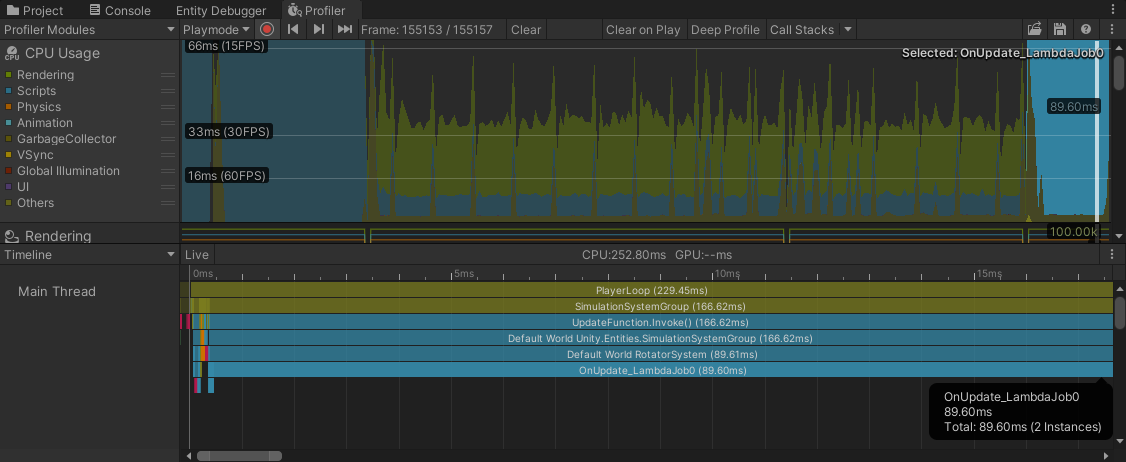
\includegraphics[width=0.95\columnwidth]{gfx/imgs/chapter5/ProfilerStressTest100k(2).png}
    \caption{Profiler: rotazione di 100.000 entità eseguendo il sistema sul main thread.}
    \label{fig:profiler-100k(2)}
\end{figure}

\subsubsection{ECS con job}
In questo test abbiamo utilizzato ECS insieme al Job System. Quindi, invece di eseguire la lambda expression del sistema \verb|RotatorSystem| sul main thread, abbiamo schedulato un job per la sua esecuzione. Così facendo possiamo scaricare il lavoro della CPU su un core secondario.
Dal Profiler possiamo vedere come la \verb|OnUpdate()| sul main thread impieghi solo 0,043 ms, con un notevole miglioramento rispetto alle due prove precedenti. Questo è dovuto al fatto che il lavoro del sistema viene scaricato su un job secondario, il quale impiega un tempo di 100 ms per essere eseguito. Così facendo otteniamo un incremento degli FPS, che raggiungono una media di 6,9 (Figura~\ref{fig:dati-stress-test}). 

\begin{figure}[!ht]
    \centering
    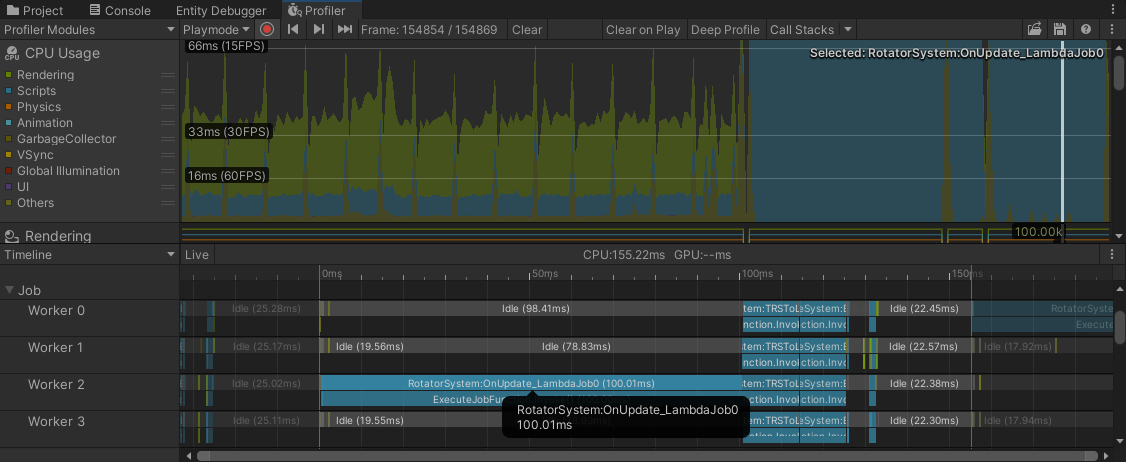
\includegraphics[width=0.95\columnwidth]{gfx/imgs/chapter5/ProfilerStressTest100k(3).png}
    \caption{Profiler: rotazione di 100.000 entità tramite scheduling di un job su un worker thread.}
    \label{fig:profiler-100k(3)}
\end{figure}

\subsubsection{ECS con job paralleli}
Come nel caso precedente, in questo test abbiamo utilizzato ECS assieme al Job System. Tuttavia, abbiamo scelto di parallelizzare ulteriormente questo meccanismo sfruttando il metodo \verb|ScheduleParallel()|. Questo metodo ci permette di distribuire il lavoro della CPU sui core secondari utilizzando i job paralleli.
Così facendo, il lavoro viene smaltito da 8 job contemporaneamente, ognuno dei quali impiega circa 147 ms per essere eseguito. Anche in questo caso, il main thread impiega circa 0,04 ms per eseguire la \verb|OnUpdate()|. Se a questo aggiungiamo una maggiore parallelizzazione, otteniamo un incremento delle prestazioni che porta l'applicazione a 13,9 FPS (Figura~\ref{fig:dati-stress-test}).

\begin{figure}[!ht]
    \centering
    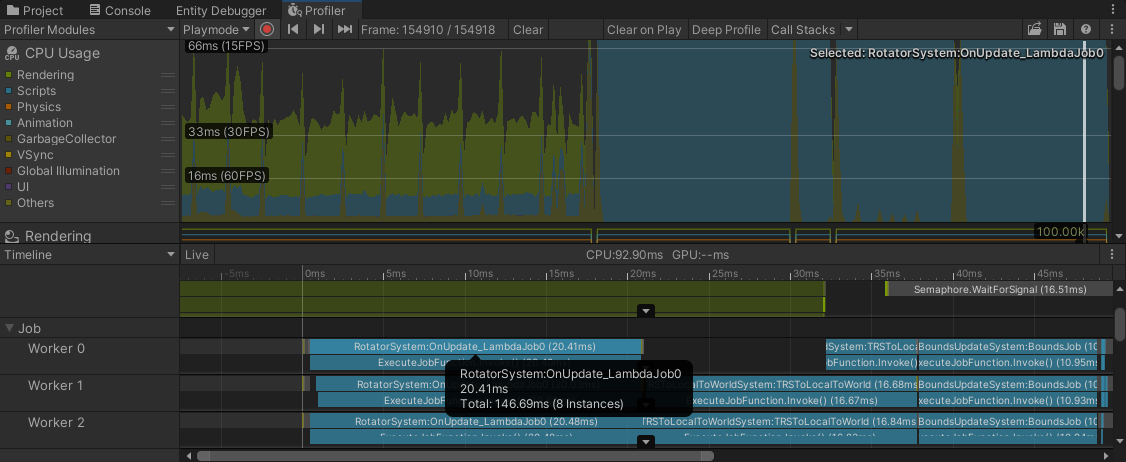
\includegraphics[width=0.95\columnwidth]{gfx/imgs/chapter5/ProfilerStressTest100k(4).png}
    \caption{Profiler: rotazione di 100.000 entità tramite job paralleli su worker thread.}
    \label{fig:profiler-100k(4)}
\end{figure}

\subsubsection{ECS con job paralleli e Burst compilation}
In questo ultimo test abbiamo sfruttato il Burst Compiler. Questo ci permette di compilare il bytecode IL/.NET dei nostri job in codice nativo estremamente performante. Infatti, semplicemente abilitando l'opzione dell'editor ``Jobs $>$ Burst $>$ Enable Compilation'', siamo riusciti ad ottenere un notevole incremento delle prestazioni: il tempo di esecuzione dei job paralleli è arrivato ad una media di circa 9,2 ms totali per 8 istanze (vedi Figura~\ref{fig:profiler-100k(5)}), mentre gli FPS a runtime sono quasi raddoppiati.

\begin{figure}[!ht]
    \centering
    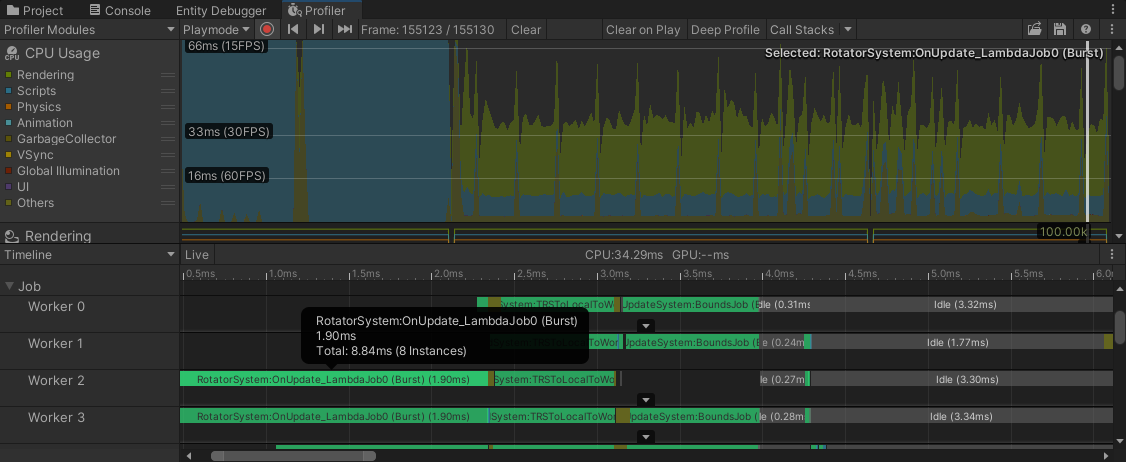
\includegraphics[width=0.95\columnwidth]{gfx/imgs/chapter5/ProfilerStressTest100k(5).png}
    \caption{Profiler: rotazione di 100.000 entità tramite job paralleli compilati con Burst su worker thread.}
    \label{fig:profiler-100k(5)}
\end{figure}


In Figura~\ref{fig:dati-fps} abbiamo riportato un grafico riassuntivo delle prestazioni in base agli FPS. In particolare, vengono paragonate tutte le implementazioni di cui abbiamo discusso in precedenza.

\begin{figure}[!ht]
    \centering
    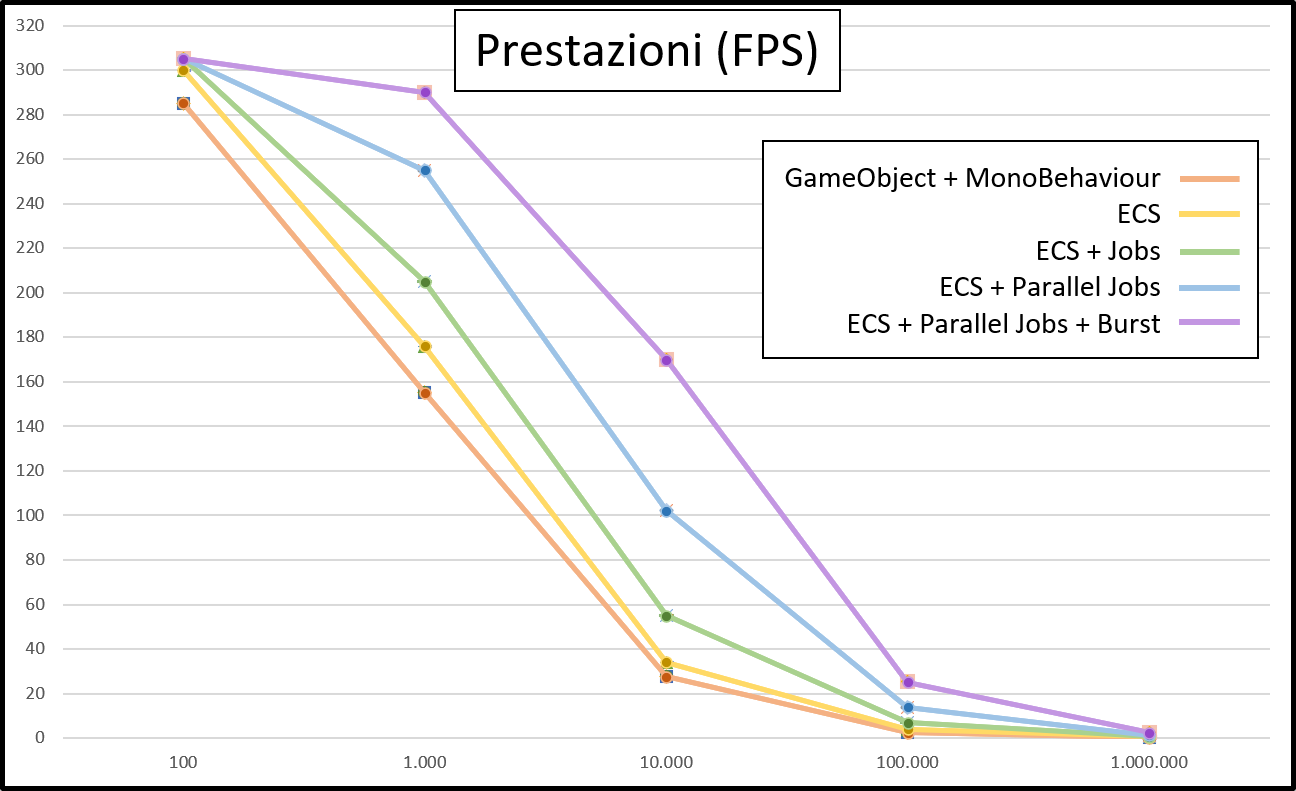
\includegraphics[width=0.95\columnwidth]{gfx/imgs/chapter5/FPSGraph.png}
    \caption{Grafico degli FPS (l'ascissa rappresenta il numero di cubi che vengono fatte ruotare, l'ordinata gli FPS relativi).}
    \label{fig:dati-fps}
\end{figure}

Dal grafico è evidente come l'utilizzo di ECS porti ad un miglioramento di prestazioni nei confronti del modello basato su GameObject. Inoltre, il divario fra le due architetture cresce all'aumentare del numero di cubi creati; soprattutto nel caso in cui utilizziamo ECS in combinazione con gli altri package.
